%!TEX root = ../template.tex
%%%%%%%%%%%%%%%%%%%%%%%%%%%%%%%%%%%%%%%%%%%%%%%%%%%%%%%%%%%%%%%%%%%%
%% chapter3.tex
%% NOVA thesis document file
%%
%% Challenges and requirements to build the DSL
%%%%%%%%%%%%%%%%%%%%%%%%%%%%%%%%%%%%%%%%%%%%%%%%%%%%%%%%%%%%%%%%%%%%




\chapter{Challenges and Requirements for a Configurable Code Generator}
\label{chap:challenges_and_requirements}

\epigraph{
	This chapter explain why configurability is no longer optional, and how traditional code generation pipelines must evolve. In addition, a prototype of the configuration is also presented along with an implementation plan.
}

\section{The Inflexibility of RAMSES: A Barrier to Industrial Integration}
\label{sec:inflexibility_ramses}

RAMSES has served as a robust model-to-code generator for AADL-based systems, yet it suffers from a fundamental architectural constraint: it assumes a uniform target environment. This assumption does not hold in real-world industrial projects, where system heterogeneity, legacy integration, and domain-specific standards define a constantly shifting context.

The core issue lies in RAMSES’ transformation pipeline: it entangles policy decisions (naming, structure, integration style) with generation logic. These decisions, hardcoded in ATL transformations, reflect the assumptions of RAMSES' authors more than the needs of end users. Altering them involves modifying the transformation source itself, often a hard and error-prone task.

Consider a simple use case: a company mandates that all task-level functions use `snake\_case` and include a `COMPONENT\_` prefix. RAMSES, which might generate `ComputeTask` by default, offers no way to enforce those rules. A change in naming becomes a traversal through ATL templates and helpers. This is not scalable, and in safety-critical software, it is not acceptable.

Furthermore, beyond naming, decisions about memory allocation models, system initialization flows, and error handling behaviors are equally rigid. There is no declarative layer that allows users to steer generation outcomes according to organizational needs or evolving constraints. As such, RAMSES provides code generation but not code governance.

\section{Industrial Realities and Pressures}
\label{sec:industrial_realities}

To understand why this rigidity is problematic, we must shift perspective from the generator to the organization that consumes it. In industry, generated code is not ephemeral: it is versioned, peer-reviewed, statically analyzed, tested, and in some cases certified. It coexists with handwritten code, interfaces with platform-specific services, and must evolve alongside requirements.

\subsection*{Compliance, Traceability, and Certification}

Generated code must often comply with domain-specific standards such as:

\begin{itemize}
	\item \textbf{\gls{MISRA} C/C++:} Imposes constraints on memory usage, naming, control flow, and portability~\cite{Misra_C_2025}~\cite{Misra_Cpp_2023}.
	\item \textbf{DO-178C:} Requires traceability, tool qualification, and clear derivation from high-level requirements. 
	\item \textbf{ISO 26262:} Enforces safety-related development practices and documentation.
\end{itemize}

In these environments, code generation must do more than "just work". It must be explainable, auditable, and deterministic. Developers must be able to trace a generated function back to a model element and forward to a specific runtime behavior.

\subsection*{Integration with Legacy Codebases}

Most industrial systems are not built from scratch. Code generators must work alongside:

\begin{itemize}
	\item Legacy libraries with non-negotiable \gls{API}s.
	\item Hardware abstraction layers that impose structural patterns.
	\item Existing software architecture rules (how modules communicate, how tasks are organized).
\end{itemize}

A code generator that cannot adapt to these constraints is often sidelined in favor of manual glue code or post-processing scripts. These scripts, in turn, introduce maintainability challenges and break traceability chains.

\subsection*{Developer Ergonomics and Maintenance}

Even the most advanced generator will eventually produce code that is read (and possibly modified) by a human developer. 

\begin{tcolorbox}[colback=green!8]
	If developers can't read or rely on the generated code, they will stop trusting it altogether.
\end{tcolorbox}

Poor formatting, ambiguous naming, or surprising control flow all reduce the utility of generated artifacts, leading teams to "lock" generated files and prohibit modifications: an anti-pattern that defeats the promise of model-driven engineering.

\section{Why Configuration Matters}
\label{sec:why_configuration_matters}

To resolve the issues above, we must introduce a new abstraction layer: one that separates \textbf{what} is generated from \textbf{how} it is generated. This is the role of a configuration language.

A configuration language provides a structured way to express \textbf{generation policy}: the set of rules, conventions, and constraints that tailor code to its industrial context. Importantly, it allows these policies to be:

\begin{itemize}
	\item \textbf{Externalized} from the transformation logic.
	\item \textbf{Composable} and layered across project variants.
	\item \textbf{Validated} for correctness before code generation begins.
\end{itemize}

Such language enables a fundamental shift: from a monolithic, one-size-fits-all generator, to a configurable and extensible platform that adapts to its environment.

\section{Characteristics of an Effective Configuration Layer}
\label{sec:config_language_characteristics}

Designing this kind of language is challenging. It needs to balance expressiveness, ease of use, and seamless integration. Based on industrial feedback and analysis of RAMSES issues, the following characteristics are proposed:

\begin{itemize}
	\item \textbf{Declarative, Not Imperative}: Users should describe \textbf{what} they want ("all functions must use snake\_case") rather than \textbf{how} to achieve it. This aligns with the model-driven philosophy and supports better configuration analysis.
	\item \textbf{Human-Readable and Tool-Accessible}: The configuration format (proposed \gls{DSL}) should work well with version control, support difference review, and remain readable to engineers. It must also be machine-readable for validation and generation.
	\item \textbf{Functionally Equal to the Default Code}: The newly generated code should remain functionally the same as without the configurator. Meaning that it should produce the same practical result with or without the configuration, excluding performance metrics.
	\item \textbf{Configures the Generator, Not the Model}: Configuration keys should influence how the code is generated, without requiring changes to the input models. The DSL operates alongside the model, guiding the generators behavior (naming, structure or implementation strategy) based on domain concepts such as \texttt{thread}, \texttt{port}, or \texttt{data component}. Configuration keys should remain semantically aligned with modeling elements but their primary role is to modify generator logic, not to modify or extend the models themselves.
	\item \textbf{Validated and Error-Tolerant}: Invalid configurations should produce clear diagnostics before generation starts. Where possible, defaults and fallbacks should be available to prevent blocking workflows.
	\item \textbf{Extensible and Portable}: The configuration will be easily extensible thanks to its Ecore background, allowing for easy inclusion of new features. At the same time, since the language model is detached\footnote{The language model (Ecore) itself is not locked exclusively to \gls{RAMSES} and can be used in other projects, however, that implies having to code the logic for each feature according to project specifics.} from \gls{RAMSES}, it can be easily included in other projects, allowing for a quicker development of a configuration language once this one is built.
\end{itemize}

These characteristics will make the configuration language robust, maintainable, and suitable for industrial use, allowing for flexible customization of code generation without compromising model integrity or introducing unnecessary complexity.

\section{Beyond Code Formatting: What Configuration Should Control}
\label{sec:config_scope}

While naming and formatting are important, a powerful configuration system must go further. The following dimensions should be within scope:

\begin{enumerate}
	\item \textbf{Artifact Naming and Structuring:} Control over file names, folder layout, and identifier styles.
	\item \textbf{Component Mapping Rules:} Declarative rules that assign AADL components to target platform concepts (RTOS tasks, processes, etc).
	\item \textbf{Code Instrumentation:} Hooks for logging, tracing, or runtime checks (insertion of `assert` or instrumentation macros).
	\item \textbf{Conditional Feature Flags:} Ability to enable or disable parts of the generator (generate test stubs, insert wrappers).
	\item \textbf{Code Documentation:} Generation of reports or toggle of code comments.
\end{enumerate}

\begin{tcolorbox}[colback=blue!5, colframe=blue!50!black, title=Configuration is More Than Style]
	While formatting is the most visible aspect of configurability, its true value lies in controlling semantic properties of the generated code: platform binding, integration, traceability, and lifecycle.
\end{tcolorbox}

\section{Proof of concept}
\label{sec:proof_of_concept}

In order to better understand the whole concept of the \gls{DSL} to be built during this thesis, a prototype that encompasses a specific feature needed in the \gls{RAMSES} tool was built with the intent of showcasing the usage of the configuration language, in a controlled environment.

\subsection{How it works}
\label{sec:how_it_works}

The selected feature to be implemented by the prototype was the Identifier Modification option, which essentially means having a higher control over the generated function, variable, and class names in the generated code. This features was chosen since it is fairly straight forward to implement and also decently portable, more on that later. 

Lets take the following example:

\begin{verbatim}
class MyNode : public rclcpp::Node {
	public:
	MyNode() : Node("my_node") {
		(...)
	}
\end{verbatim}

A simple Node class has the class identifier \texttt{MyNode}. In the case of \gls{RAMSES}, MyNode would be inherited from the AADL model, meaning that, in order to change the code nomenclature of MyNode, we would have to either manually change the generated code or changing the name of the node in it's corresponding AADL model file and then regenerate the code.

Both options are feasible in this case, however, with growing system complexity this small change becomes incrementally harder and more prone to errors.

The developed prototype focuses directly on that front, providing an adjacent configuration model that works alongside the main one with the goal of delivering that missing configuration option, here's how it works:

\begin{enumerate}
	\item The placeholder code is built, in this case it was from a taskset style project\footnote{This project is a \gls{DSML} that communicates task sets and automatically generates C code using Acceleo, targeting the RT-POSIX real-time gls{API}.}
	\item The target naming convention is selected in the configuration model
	\item The final code is generated with the now correct identifier nomenclature.
\end{enumerate}
 
 
For a clearer understanding of the flow of the prototype, here's a flowchart:

\begin{figure}[htbp]
	\centering
	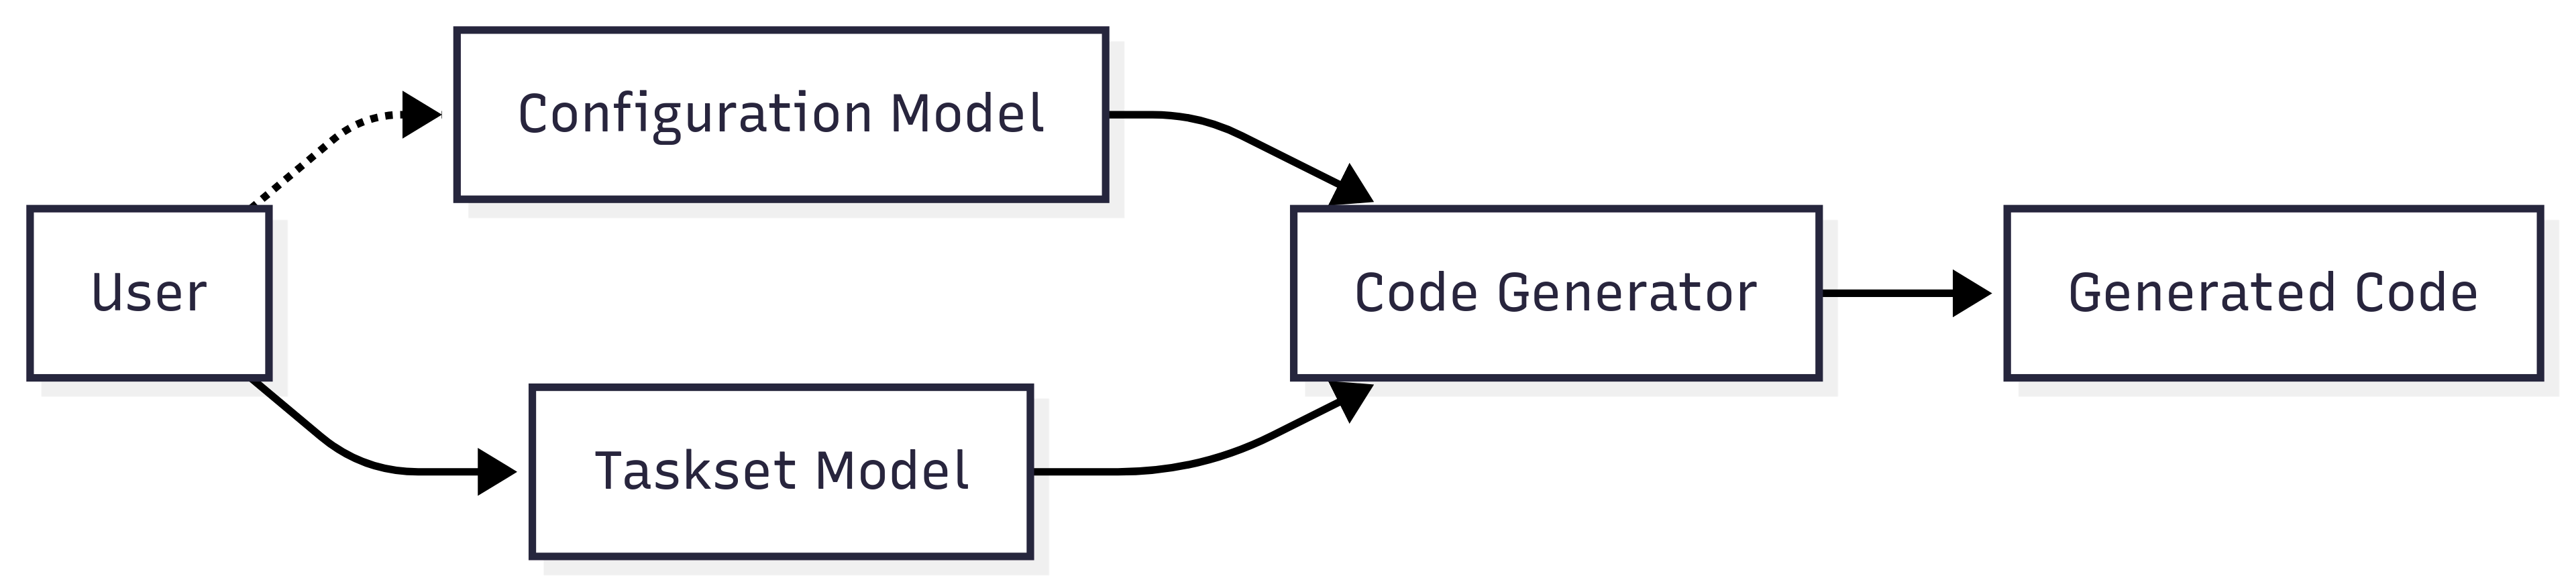
\includegraphics[height=0.22\textwidth]{prototype_flowchart.png}
	\caption{Flowchart of the prototype}
	\label{fig:prototype_flowchart}
\end{figure}

The user interacts with the main model (Taskset in this case) and \textit{can} interact with the configuration model aswell, if thats the case, the user will see changes in the code in accordance to the options selected in the configuration model.

The configuration model is not tightly coupled to the main workflow and is not mandatory, it works alongside the main model but provides extra options and choices to the user in therms of code customization, effectively elevating a bit more the code quality of the given taskset generated code.

\subsection{Practical Example}
\label{sec:practical_example}
 
Let's take a look at a practical example of the prototype, and, since the placeholder code has already been defined and altered to allow for dinamic identifier changes, all we have to do is select the naming convention on the configuration model.

\begin{figure}[htbp]
	\centering
	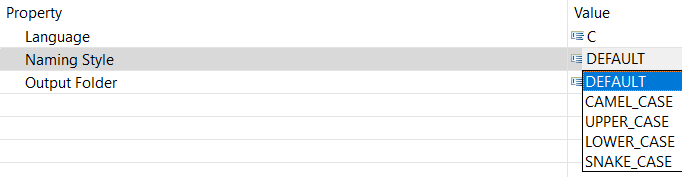
\includegraphics[height=0.22\textwidth]{naming_convention_selection.png}
	\caption{Selection of the naming convention}
	\label{fig:prototype_selection}
\end{figure}

As we can observe from Figure~\ref{fig:prototype_selection}, the prototype presents a rough and unrefined way of user interaction, in order to change the configuration the user must change the configuration model itself via its properties, which is not the end goal for the final product but works well in testing/controlled environments. 

The current selected option in Figure~\ref{fig:prototype_selection} is the default option, which will not modify the file:

\begin{figure}[htbp]
	\centering
	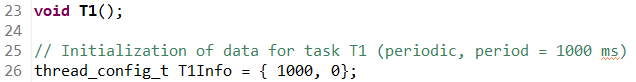
\includegraphics[height=0.12\textwidth]{default_naming_option.png}
	\caption{Result of the code generation in the default form}
	\label{fig:prototype_default_option}
\end{figure}

Taking in the result from Figure~\ref{fig:prototype_default_option} we can get an idea of the default, unaltered code generation, but our goal is not simply to generate code, we can select a different naming option via the configurator model, save, and regenerate the code. The change is clear.

\begin{figure}[htbp]
	\centering
	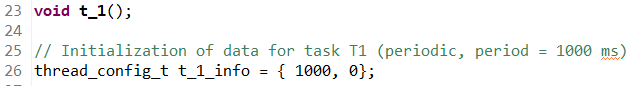
\includegraphics[height=0.12\textwidth]{snake_case_naming_option.png}
	\caption{Result of the code generation with the snake\_case naming option}
	\label{fig:prototype_snake_case}
\end{figure}

Comparing Figure~\ref{fig:prototype_default_option} with Figure~\ref{fig:prototype_snake_case}, we can clearly see where the configuration model applies its modifications: always on the identifiers and never on anything else, especially not on the keywords\footnote{Keywords like \textit{Void} are common and easy to identify. In this observed case however, in both Figures~\ref{fig:prototype_default_option} and~\ref{fig:prototype_snake_case} we see that \textit{thread\_config\_t} is also present but this is a \textit{Struct}, which, while not an exclusive keyword, it serves a purpose like \textit{Void} or \textit{int} and is \textbf{not} an identifier.}.

The idenfitiers (in this case the name of the function\footnote{T1} and the name of the variable\footnote{t\_1\_info}) change seamlessly according to the selected naming convention in the configurator. This is the expected behaviour for the features to be implemented, they should provide additional value while also keeping the base generated code available if the user does not wish to modify it at all. 

\subsubsection{User Feedback}

In order to test the functionality and receive a third party opinion, a simple user testing was done with multiple users that were familiar with AADL. The procedure was simple and direct, users were instructed to the premise of the prototype, then they would perform tasks (in this case just one task: change the identifier name to X) and then they would be questioned in the usefulness of the feature, the applications it could have and overall thoughts.

Upon doing this testing, many users defined it as a flexible addition to coding generation with many application to real life and industry scenarios. Users also noted that this functionality improves information treatment between teams as different people have different ways to write models names, the prototype proves that naming normalization can also improve team cohesion.

Users commented that, with this functionality, appears the ability to create multiple versions of the functionally same code just with naming differences. This also aligns with the coding standards for multiple languages, given that some languages require identifiers to use a certain nomenclature, which can clash with AADL node names.

Overall the prototype, although simple, was well received and proved to give value for the AADL to code pipeline.

\subsection{Technical Details}
\label{sec:prototype_technical_details}

Even though its application is specific to the code developed for the prototype is fairly generic. This means that, most of the logic and code used for this prototype can be ported directly to RAMSES without much issue, effectively implementing the feature, albeit testing will still be performed.

The naming convention change logic is pretty straight forward, as we want to modify the identifiers, and those come from model properties. From there the properties that represent identifiers are formatted as they are being added to the code, effectively making sure the main model stays untouched while the properties extracted are modified into the desired outcome. This makes sure only the specific selected properties are modified and the rest of the code generates as normal.

The algorithm used for the naming transformation has many fallbacks that make it so even if a property name is especially complex, cases like short names are handled with care and specific styles like snake\_case, while having complex patterns, can be easily defined with Regex lines. 

As the configuration model is built on Ecore, the addition of new naming styles is not possible directly by the user, this means two things: in order to enter a wrong coding style the user needs to have high technical knowledge of the system\footnote{This can change with the proper DSL implementation, however, configuration checks will be applied then, removing this problem.}. If instead we wanted to \textbf{add} a new naming style, that is very much possible with a quick modification of the Configurator's Ecore model and the Acceleo naming format algorithm.

\subsubsection{Multiple Models in Acceleo}

Working with 2 Ecore models was not very straightforward, although Acceleo provides the resources needed to work with multiple Ecore models, Eclipse itself does not allow for multiple input models in a single run configuration. To work around this, a custom \textit{main()} method was made to register the metamodels into the resources, effectively allowing for the usage of both metamodels. This issue, while small, presented a fairly decent deal of complications for the development of the prototype, specifically because Acceleo documentation on the matter was scarce and community forums were unhelpful.

Nevertheless, this solution allows not just for the usage of multiple models in this prototype but also in any other projects that need an Acceleo program with 2 or model Ecore models as inputs.


\section{System Evaluation}
\label{sec:sys_eval}

In order to assure that the \gls{DSL} meets expectations, the system will be evaluated in various forms, mainly:

\begin{itemize}
	\item The \gls{DSL} exists and produces results.
	\item Before and after comparison (with code configurator vs without).
	\item Usability evaluation.
	\item Configuration variants evaluation.
	\item The newly generated code remains functionally the same as before\footnote{Meaning that it performs the same practical task as before the \gls{DSL} implementation.}.
\end{itemize}

Ideally the end product should meet these requirements to be considered a success. Each one of the requirements ensures a different, core quality of the configuration system, such as correctness, usability, or robustness.

\subsection*{DSL existence}

This requirement will be fairly straightforward to prove since it implies a direct usage of the \gls{DSL} in order to produce results. This can be proven alongside the other requirements as they depend on it, however, a system wide testing will quickly prove the existence of the configuration language and its impacts, specifically with the testing of all features developed and their results.

\subsection*{Before and After Comparison}

The core idea of this configuration language is to modify the output code of the code generator according to user needs. The best way to prove that this goal was achieved is to compare how users would perform the same task before the configuration language was implemented and after. This direct comparison will evaluate the direct impact of the configuration language on development and will ensure that the developed solution benefits the system. 

\subsection*{Usability}

The configuration language should be easily usable, even by end users with limited programming experience, in order to ensure this requirement is met, clear documentation, consistent syntax, and terminology aligned with the application domain should be prioritized. This requirement will be confirmed by comparing the interaction with the configuration language of users with varying levels of technical expertise, allowing the comparison of usability and learning curve.

\subsubsection*{User Evaluation Methodology}

Participants will be given predefined configuration tasks (changing naming schemes, visualizing traceability, etc) and asked to perform them with minimal guidance.

The evaluation will collect both quantitative and qualitative data:
\begin{itemize}
	\item Task completion time
	\item Number and type of errors
	\item Subjective feedback on ease of use
	\item Observed learning curve
	\item Type and gravity of misunderstandings
\end{itemize}

This setup will help assess whether the DSL meets its usability goals across a broad user spectrum.

\subsection*{Configuration Variants}

To assess the flexibility and robustness of the configuration language, distinct configuration files will be tested. These scenarios will vary in complexity and structure to evaluate whether the generator can handle diverse inputs while maintaining correctness and coherence in the generated code. Effectively testing the limits of the configuration language.

\subsection*{Functionally Equal}

To make sure the code generated still retains the same practical functionality, a few things need to be taken into account, firstly, the code generator needs to be modified just enough to produce the desired results of structure, naming, etc while still keeping the same functionality as before the implementation, essentially keeping the semantics intact. Monthly testings will also ensure that the code remains functionally the same by running selected examples and doing direct code comparison, however, comparisons will focus on runtime behavior rather than raw text equivalence. 


The baseline for comparison will be the unmodified RAMSES generator. This allows for a clear assessment of what configuration capabilities are introduced in terms of productivity, flexibility, and clarity.


\section{Research Limitations}
\label{sec:research_limitations}

Although the configuration language includes many features and has been designed with flexibility, usability, and maintainability in mind, this work has some limitations.

\begin{itemize}
	\item \textbf{Limited Scope of Configurable Aspects:} The proposed DSL focuses primarily on naming conventions, traceability, and coding standards. More advanced features such as behavioral configuration, cross-component constraints, or real-time performance tuning fall outside the scope of this work. Similarly, certain features might be prioritized or excluded based on client feedback.
	
	\item \textbf{Restricted Evaluation Sample:} Usability and functional testing rely on a small set of representative examples and a limited number of user interactions. While including users with varying levels of technical expertise is being kept in mind, the results may not generalize across all industrial contexts or teams.
	
	\item \textbf{No Legacy Tool for Direct Comparison:} Since no previous configuration language exists for \gls{RAMSES}, or AADL for that matter, before and after comparisons will rely on manual, potentially subjective assessments of workflow complexity. This limits the ability to measure productivity gains with high precision.
	
	\item \textbf{Integration Constraints:} The configuration system is designed to integrate into the existing \gls{RAMSES} toolchain, which constraints how the generator behavior can be modified. Deep generator reworks or architectural transformations are intentionally excluded to maintain compatibility.
	
	\item \textbf{Scalability Not Fully Tested:} The \gls{DSL} should performs well on example models, its performance and maintainability might not be validated on extremely large or complex input systems, which are typical in some industrial environments. This might not be a constraint if such models are later used for testing.
	
\end{itemize}

These limitations do not compromise the core contributions of this work, but they highlight areas for future development, such as broader configuration domains, wider user studies, and deeper toolchain integration.


\section{Toward a Generator for System Integrators}
\label{sec:conclusion_configurable_generation}

RAMSES has proven to be a robust and effective tool for model-to-code generation, particularly within academic contexts and controlled environments. However, as embedded systems development increasingly intersects with regulatory and industrial demands, the expectations placed on code generators have grown. Beyond correctness, they must now offer adaptability, traceability, and long-term maintainability to meet evolving project requirements.

Introducing a configuration language is not merely a feature, it's an architectural shift. It allows users to define their generation context without touching generator internals, reducing risk, increasing reuse, and enabling automation across product lines.












